\documentclass[twoside]{article}
\usepackage[utf8]{inputenc}
\usepackage[T1]{fontenc}
\usepackage[french]{babel}
\usepackage{aeguill}
\usepackage{actes}
\usepackage{amsmath}
\usepackage{amsthm}
\usepackage{amssymb}
\usepackage{stmaryrd}
\usepackage{url}
\usepackage{hyperref}
\usepackage{xypic}
%\CompileMatrices
\usepackage{mathpartir}
\usepackage{graphicx}

\newcommand{\liquidsoap}{Liquidsoap}
\newcommand{\savonet}{Savonet}
\newcommand{\eg}{e.g.~}
\newcommand{\cf}{cf.~}
\newcommand{\letin}[3]{\text{\texttt{let }} #1 = #2 \text{\texttt{ in }} #3}
\newcommand{\univ}[2]{\forall #1.~ #2}
\newcommand{\regle}[1]{\text{\textrm{(#1)}}}
\newcommand{\mabs}[2]{\lambda\{#1\}.#2}
\newcommand{\tmabs}[2]{\{#1\}\to #2}
\newcommand{\mapp}[2]{#1\{#2\}}
\renewcommand{\vec}[1]{\overrightarrow{#1}}
\newcommand{\TODO}[1]{\textbf{TODO~: }{#1}}
\newcommand{\FV}[1]{\mathcal{FV}(#1)}
\newcommand{\eqdef}{:=}
\newcommand{\interp}[1]{\llbracket{#1}\rrbracket}

\title{De la webradio lambda à la $\lambda$-webradio}

\author{D. Baelde$^1$
        \& S. Mimram$^2$}

\titlehead{De la webradio lambda à la $\lambda$-webradio}

\authorhead{Baelde \& Mimram}% a gauche (page paire)

\affiliation{\begin{tabular}{rr}
\\ 1:  INRIA \& LIX, \'Ecole Polytechnique
\\     {\tt david.baelde@ens-lyon.org}
\\ 2:  \'Equipe PPS, CNRS / Université Paris 7
\\     Case 7014, 75205 Paris cedex 13
\\     {\tt samuel.mimram@ens-lyon.org}
\end{tabular}}

\hypersetup{
  pdftitle={De la webradio lambda à la lambda-webradio},
  pdfauthor={David Baelde et Samuel Mimram},
  unicode=true,
  colorlinks=true,
  linkcolor=black,
  citecolor=black,
  urlcolor=black
}

\theoremstyle{plain}
\newtheorem{proposition}{Proposition}
\newtheorem{lemme}{Lemme}
\theoremstyle{definition}
\newtheorem{definition}{Définition}
\theoremstyle{remark}
\newtheorem{exemple}{Exemple}
\newtheorem{remarque}{Remarque}

\begin{document}
\setcounter{page}{1}
\maketitle

\begin{abstract}
  La génération et la manipulation de flux audio -- pour une radio \emph{web}
  par exemple -- est une tâche complexe, difficilement réalisable à l'aide des
  langages de programmation habituels. Nous présentons dans cet article un
  langage fonctionnel fortement typé appelé \liquidsoap{} qui offre des
  abstractions confortables pour décrire la construction de flux élaborés.
  Il se démarque par sa souplesse d'utilisation et
  la richesse des possibilités qu'il offre~:
  de l'utilisation de divers types d'entrées
  (fichiers audio, micro, requêtes d'utilisateurs)
  que l'on peut sélectionner dynamiquement
  (selon la disponibilité ou encore l'horaire)
  à la gestion des transitions entre morceaux et autres traitements audio.
  % sans oublier diverses interfaces avec l'exterieur: scheduler externe,
  % telnet, site web, server de diffusion
  La nécessité d'avoir un
  langage riche et abordable nous a amenés à introduire une variante
  du $\lambda$-calcul typé, avec étiquettes et arguments optionnels,
  dont la portée va au delà du domaine du traitement audio.
\end{abstract}

% \tableofcontents
% \newpage

Avec l'avènement des réseaux à haut débit, il est maintenant possible de
diffuser rapidement de grandes quantités de données à travers le monde. Ainsi,
de nombreuses radios \emph{web} ont pu voir le jour et diffusent en continu
divers contenus sonores par le biais d'Internet. Il n'existait cependant pas de
langage simple et expressif permettant de construire les flux audio de ces
radios.

Au premier abord, la génération d'un flux continu de données audio peut sembler
être une tâche simple à réaliser~: il suffit de lire bout à bout des fichiers
audio. Cependant, sa mise en pratique se heurte rapidement à certaines
difficultés.
\begin{itemize}
\item Ces difficultés sont d'abord d'ordre purement technique~: les fichiers
  audio sont stockés sous divers formats (il faut les convertir en un format
  uniforme), sur divers serveurs (il faut des outils gérant les protocoles
  utilisés), etc.
\item Ensuite, la gestion des listes de lecture, ou \emph{playlists}, s'avère
  complexe~: on veut pouvoir choisir un morceau correspondant à certains
  critères (le titre, l'artiste, le genre, etc.) dans une base de données, ces
  critères dépendant de l'horaire (on veut jouer de la musique douce le matin et
  plus dansante le soir), on veut aussi pouvoir avoir des interventions en
  direct lors de plages horaires réservés aux animateurs,
  insérer régulièrement des messages rappelant le nom de la radio
  (\emph{jingles}), etc.
\item Enfin, il faut pouvoir traiter le son provenant des fichiers audio afin de
  le rendre uniforme et agréable à l'écoute~: il faut à la fois appliquer des
  effets audio sur le son (en particulier normaliser et compresser le son afin
  d'avoir un volume moyen constant), gérer l'enchaînement entre les morceaux
  (par exemple, appliquer un fondu enchaîné entre les chansons), éviter les
  blancs, etc.
\end{itemize}

Il existait déjà plusieurs logiciels qui permettent de gérer des radios.
%
Les solutions les plus professionelles
(Master~Control, WinRadio, Open~Radio ou encore Rivendell)
sont des applications graphiques intégrant la gestion de la grille de 
diffusion, le contrôle des points de transitions entre fichiers,
le décrochage vers une émission en direct et enfin la diffusion.
%
D'autres applications plus spécialisées et légères, 
ont une interface en mode console et sont plus adaptées à un fonctionnement 
complètement automatisé sur un serveur.
Ces derniers générateurs de flux (par exemple Ices ou EzStream)
offrent des possibilités limitées à la diffusion d'une suite de fichiers sans 
transitions ou d'un flux en provenance de la carte son.
Ils sont cependant très utilisés dans la communauté
\emph{open-source}, notamment dans le système Mediabox~404 qui offre une 
interface web conviviale permettant de gérer une grille de diffusion et le 
décrochage vers les émissions en direct.
%
Dans tous les cas on remarque que la génération du flux se fait selon un schéma
rigide~: l'ordre dans lequel les opérations sont effectuées est fixe. Ces outils
ne sont par conséquent plus utilisables dès que l'on sort du cadre pour lequel
ils ont été conçus.

% On manque ainsi d'un système générique permettant de décrire des
% configurations adaptées à toutes sortes de besoins.

La conception d'un langage applicatif dédié, fournissant
des opérations élémentaires sur des valeurs représentant les flux,
offre un cadre de développement riche ainsi qu'un moyen simple et expressif
pour l'utilisateur de décrire sa configuration. Nous présentons ici le langage
\liquidsoap~\cite{savonet}, une implémentation de cette idée en
OCaml~\cite{ocaml}. Cet outil offre de larges possibilités
et est d'ores et déjà utilisé avec succès en production par des
webradios~\cite{dolebrai,radiopi} ou encore pour expérimenter de nouvelles
méthodes de diffusion, par exemple fondées sur le recoupement des habitudes
musicales de groupes d'auditeurs \cite{baccigalupo-plaza:song-scheduler}.

L'une des contraintes majeures qu'un tel langage doit respecter, au delà de
celles induites par la manipulation de flux audio, est liée à la nature des
utilisateurs potentiels~: les personnes susceptibles de vouloir créer des radios
sur internet sont loin d'être toutes des programmeuses chevronnées. Nous avons
donc conçu le langage de sorte qu'il soit abordable et simple d'utilisation. En
particulier, le grand nombre de paramètres dont peuvent dépendre les opérations
du langage nous a amené à introduire un calcul avec étiquettes (ce qui permet
à l'utilisateur de ne pas avoir à se souvenir de l'ordre des arguments) et
arguments optionnels (permettant de spécifier des valeurs par défaut pour les
arguments) ainsi qu'un système de types pour ce calcul, qui sont deux
contributions originales de cet article. Ce calcul n'est pas spécifique au
traitement de l'audio et peut être réutilisé dans d'autres domaines où la
simplicité du langage passe avant la nécessité d'une compilation efficace, par
opposition avec les calculs développés par Aït-Kaci, Garrigue et
Furuse~\cite{ait-garrigue:label,furuse-garrigue:labelopt}.

% Précisons qu'on ne va pas parler de cambouis, sisi.
Nous abordons dans cette article deux aspects fondamentaux de la conception de
\liquidsoap{}.
Nous commençons par présenter les abstractions fournies dans
le langage en illustrant les possibilités qu'elles offrent
et nous discutons de l'adéquation entre ces abstractions et l'implémentation.
Dans un second temps, nous formalisons le calcul sous-jacent au
langage de programmation ainsi qu'un système de types adapté.

\section{Un langage de manipulation de flux audio}
\label{sec:flux}
Notre présentons ici la méthodologie et les concepts généraux importants qui
sous-tendent le langage. Nous nous sommes efforcés d'être synthétiques,
le lecteur pourra trouver plus de détails pratiques sur le site dédié au
langage~\cite{savonet}. Il est cependant intéressant de donner tout d'abord une
rapide idée de l'ampleur du développement qui a été nécessaire pour implémenter
ce langage.

Le développement de \liquidsoap{} a été effectué au sein d'un projet appelé
\savonet{} qui, outre le langage de programmation \liquidsoap{} lui-même,
contient des librairies en OCaml interfaçant des libraires C préexistantes
qui permettent de décoder et d'encoder des fichiers audio aux formats Ogg/Vorbis,
\textsc{mp3} et \textsc{aac}, d'appliquer des effets audio (greffons
\textsc{ladspa} pour les effets audio, samplerate pour changer la
fréquence d'échantillonage, etc.), de communiquer avec les cartes son
(librairies \textsc{ao}, \textsc{alsa} et portaudio), avec des programmes
externes (\textsc{jack}), ou d'envoyer le flux audio à un serveur d'émission
audio utilisant le protocole \textsc{shout}cast (Icecast par exemple).
D'autres programmes de \savonet{} permettent de créer une base de données des
fichiers audio disponibles sur un réseau ou de gérer les requêtes d'utilisateurs
via un site web ou un bot \textsc{irc} -- on peut par exemple dire «~mets
de la techno~» sur un forum de messagerie instantanée et une chanson de techno,
trouvée dans la base de donnée, sera diffusée sur la radio.

Le projet dans son ensemble comporte plus de 50~000 lignes de code dont 40~000
sont écrites en OCaml, et 8~000 en C. Le langage \liquidsoap{} lui-même comporte
25~000 lignes en OCaml. Malgré le lourd travail d'interfaçage de librairies C,
le choix d'OCaml semble avoir été fortement positif~: l'expressivité et les
capacités d'abstraction offertes par le langage nous ont permis de structurer
fortement \liquidsoap{}, de le maintenir et de l'étendre à moindre coût. En
particulier, l'utilisation intensive de la programmation objet nous a permis une
grande simplicité et extensibilité de la conception des opérations sur les flux.

% Il n'existait aucun langage capable de réaliser toutes ces tâches. Certains
% logiciels apportent cependant des solutions partielles. MediaBox
% 404~\cite{mediabox404}, qui est une interface web qui permet de gérer des listes
% de lecture, n'est pas capable d'agir directement sur l'audio (et en particulier
% de faire des transitions et d'appliquer des effets)~;
% GStreamer~\cite{gstreamer}, qui est une librairie permet de gérer des flux
% audio, est difficile à manipuler et ne gère pas les listes de lecture et
% l'émission du flux~; ChucK~\cite{chuck}, qui est un langage de programmation
% synchrone fortement typé, permet principalement de faire de la synthèse audio et
% son utilisation nécessite de comprendre comment fonctionne la programmation
% synchrone.

\subsection{Génération de flux audio dans \liquidsoap}

Un programme \liquidsoap{} construit des générateurs de flux audio: les 
\emph{sources}. Une source peut être décrite par un graphe orienté acyclique,
dont les sommets sont appelés \emph{opérateurs}.
Les sommets initiaux de ce graphe
génèrent un flux à partir d'un fichier audio, d'une liste de lecture ou 
encore d'un microphone.
Les sommets internes correspondent à des manipulations opérées sur les flux
produits par les sources filles, par exemple la superposition de ces flux, ou
le choix entre l'un d'entre eux en fonction de certains paramètres comme l'horaire ou
encore l'application d'un effet audio.
Les sommets terminaux n'ont typiquement qu'une entrée, et transmettent par 
exemple leur flux à un serveur de diffusion sur Internet ou à une carte son.
Les opérateurs, en plus de dépendre d'autres
sources décrites dans le graphe, peuvent dépendre de valeurs données en
paramètres (booléens, entiers, flottants, fonctions, etc.).

À partir d'un tel graphe, décrit par un programme \liquidsoap{}, un flux audio
est généré par blocs de données audio. Régulièrement, un bloc est décodé à
partir d'une source, des opérateurs procèdent à diverses manipulations sur ce bloc,
puis il est encodé dans un format compressé avant d'être transmis à un serveur
qui se charge de diffuser le flux aux auditeurs.
Par exemple, le programme
suivant lit des morceaux dans une liste de lecture appelée \texttt{liste} puis
applique une normalisation de volume et enfin envoie le flux à un serveur de
diffusion~:
\begin{verbatim}
l = playlist("liste")
s = normalize(l)
output.icecast.vorbis(host="www.radio.com", name="ma_radio", s)
\end{verbatim}
Le graphe induit par ce script est~:
\[
\xymatrix{
  *+[F]{\mathtt{playlist}}\ar[r]&
  *+[F]{\mathtt{normalize}}\ar[r]&
  *+[F]{\mathtt{output.icecast.vorbis}}\\
}
\]

Il nous faut enrichir la notion de flux audio pour pouvoir décrire
les configurations usuellement rencontrées.
D'une part, certaines sources ne sont pas \emph{disponibles} en permanence,
c'est-à-dire qu'elles ne sont pas tout le temps prêtes à générer des données.
Par exemple, une source jouant des requêtes d'auditeurs n'est disponible
que s'il y a effectivement des requêtes. Lorsque ce n'est pas le cas, il
faut pouvoir jouer à la place le flux provenant d'une autre source, typiquement
une liste de lecture. Si la source de requêtes devient disponible à nouveau, on
ne veut en général pas interrompre le morceau en cours mais attendre qu'il soit
terminé avant de jouer la nouvelle requête. Il faut donc d'autre part introduire une
notion de \emph{piste} dans le flux qui permette de délimiter les portions
faisant partie d'un même morceau.

\liquidsoap{} permet ainsi de décrire des opérateurs plus complexes comme
l'opérateur de choix par défaut \texttt{fallback},
qui prend en argument une liste
de sources et produit en sortie une piste de la première source disponible,
puis à la fin de celle-ci une nouvelle piste de la première source disponible
à ce nouvel instant et ainsi de suite. Il permet de réaliser ainsi notre exemple:
\begin{verbatim}
f = fallback([request.queue(), playlist("liste")])
\end{verbatim}
Le graphe sous-jacent à ce programme est:
\[
\xymatrix{
  *+[F]{\mathtt{request.queue}}\ar[r]&*+[F]{\mathtt{fallback}}\ar[r]&\\
  *+[F]{\mathtt{playlist}}\ar[ur]&\\
}
\]

Le langage permet de construire des sources encore plus élaborées. Nous
présentons dans la section suivante l'exemple de l'utilisation des transitions
entre pistes, car elle nous semble être une bonne illustration de l'expressivité
du langage et motive son caractère fonctionnel.

\subsection{Les transitions}
\label{section:transitions}
L'opération de fondu enchaîné consiste à faire varier progressivement le volume
de $0\%$ à $100\%$ (resp. de $100\%$ à $0\%$) en début (resp. en fin) de
piste. Le fondu enchaîné et croisé consiste de plus à superposer une portion de
la fin d'une piste avec le début de la précédente. Cet effet est communément
utilisé pour rendre l'écoute plus agréable. De nombreux paramètres sont à
prendre en compte~: la durée du fondu en début et en fin de piste, la durée de
la superposition ou le type de fondu (linéaire ou logarithmique par exemple),
etc. De plus, on veut parfois adapter ces paramètres en fonction des volumes
sonores, par exemple pour éviter de masquer un début de piste doux en le mixant
avec une fin bruyante. Enfin, il est aussi fréquent d'ajouter un \emph{jingle}
durant la transition.

Une solution élégante et générale pour traiter tous ces cas est de décrire une
transition par une fonction, qui prend en argument deux sources représentant les
pistes à combiner et retourne une source qui est le résultat de la
transition. Les opérations usuelles sur les flux sont alors à la disposition de
l'utilisateur pour décrire sa transition.

Par exemple, le code suivant permet d'effectuer une transition simple entre deux
pistes consécutives d'une source \texttt{s}~:
\begin{verbatim}
s = fade.out(duration=3., s)
s = fade.in(duration=2., s)
fader = fun (a,b) -> add([a,b])
cross(duration=2., fader, s)
\end{verbatim}
Dans ce programme, l'opérateur \texttt{fade.out} applique une diminution de
volume linéaire durant les trois dernières secondes d'une piste, pour arriver au
volume nul~; l'opérateur \texttt{fade.in} agit similairement mais en début de
piste. La seconde définition de \texttt{s} masque la première, le \verb.=. de la
syntaxe concrète étant à lire comme un \verb.let. dont le \verb.in. est
implicite. La fonction \texttt{fader} est ensuite définie pour décrire comment
va se faire la transition entre les pistes. Son premier paramètre sera un
tronçon de flux à croiser en fin de piste, le second paramètre correspondra au
flux commençant à la piste suivante. Ici, on se contente de superposer les deux
pistes grâce à l'opérateur \texttt{add} mais on aurait aussi pu ajouter un
\emph{jingle} durant la transition en utilisant la fonction
\verb+fader = fun (a,b) -> add([a,once(jingles),b])+. Enfin, l'opérateur
\texttt{cross} va jouer le flux en appliquant la transition
à chaque changement de piste~: à deux secondes de
la fin d'une piste, la fonction de transition est utilisée pour calculer
l'enchaînement des pistes. Graphiquement, après la première et la deuxième ligne
du script, le volume de deux pistes consécutives sera respectivement:
\begin{center}
  \begin{tabular}{ll}
    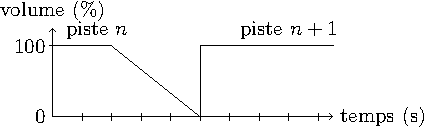
\includegraphics{transitions-out.pdf}
    &
    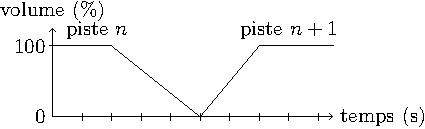
\includegraphics{transitions-out-in.pdf}
    \\
  \end{tabular}
\end{center}
Enfin, à la fin du script, après l'utilisation de l'opérateur \texttt{cross},
l'enchaînement entre pistes sera schématiquement~:
\begin{center}
  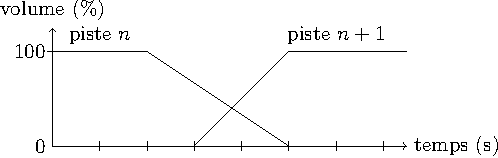
\includegraphics{transitions.pdf}
\end{center}

% La description initiale d'une source par un graphe orienté n'est plus pertinente,
% car trop statique: désormais, le graphe peut se reconfigurer dynamiquement par 
% l'application des transitions.

L'opérateur \verb.cross. doit fournir en même temps
à sa fonction \verb.fader. des données provenant de la même source \verb.s. 
mais correspondant à des instants différents dans le flux.
Il doit donc récupérer en avance et stocker les données à superposer.
Si un autre opérateur \verb.t. accédait à la source \verb.s., il 
faudrait stocker ses anciennes données pour pouvoir fournir des 
réponses cohérentes à \verb.t.. Sans hypothèse simplificatrice, ceci est 
irréalisable: la quantité de données à stocker croît sans cesse.
Dans \liquidsoap, on choisit d'exclure complètement cette possibilité:
aucune des sources en amont d'un opérateur \verb.cross. ne doit
être accédée par un autre opérateur.
Malheureusement,
c'est encore à l'utilisateur de vérifier cette condition,
en attendant une extension adéquate du système de types (cf. Section 
\ref{sec:raffinements}).

Pour finir, notons que cette représentation des transitions motive pleinement
la conception de \liquidsoap{} comme un langage fonctionnel~: contrairement à de
nombreux langages spécialisés (\emph{Domain Specific Languages}), la notion de
fonction est essentielle dans \liquidsoap{}. En effet, on ne peut pas éliminer 
les fonctions par une première passe d'évaluation partielle, car leur 
exécution est étroitement liée au processus infini de génération de flux.
%  si on avait pas l'hétérogénéité liq/ocaml on pourrait peut etre envisager
%  une optim (le coup de l'eval partielle) pour le cas où la transition n'est 
%  pas choisir dynamiquement
% Chaque appel de la fonction de transition peut produire une source au
% comportement différent. Par exemple, la fonction de transition suivante permet
% d'appliquer un fondu entre deux pistes successives uniquement si leurs volumes
% sont proches. Elle est utilisée par l'opérateur \verb.smart_cross. qui est
% similaire à \verb.cross. mais renseigne sa fonction de transition sur les
% niveaux sonores des pistes ainsi que leurs méta-données.
% \begin{verbatim}
% def transition(a,b,   # Volumes sonores avant/après
%                ma,mb, # Meta-données avant/après
%                sa,sb) # Sources avant/après
%   if   # Si les volumes sont proches et pas trop élevés...
%     a <= medium and b <= medium and abs(a - b) <= margin
%   then # ...on applique un fondu croisé.
%     add(fade.out(sa),fade.in(sb))
%   else # Sinon, on n'applique aucune transition.
%     sequence([sa, sb])
%   end
% end
% s = smart_cross(transition,s)
% \end{verbatim}
% On comprend alors bien 

\subsection{Granularité, efficacité et partage}

Nous avons décrit un système expressif pour construire un flux, en composant
des opérations élémentaires prédéfinies. Nous
discutons ici de l'écart entre la notion abstraite de flux que
l'utilisateur manipule, et son implémentation.

Précisons le cadre dans lequel se situe \liquidsoap{}, ses objectifs, sa
\emph{granularité}, par comparaison avec les
\emph{langages synchrones}~\cite{benveniste-berry:synchronous} dans lesquels
l'évaluation se fait régulièrement, et de façon théoriquement instantanée,
à chaque tic d'une horloge globale.
Il existe de tels langages dédiés à la synthèse audio, ChucK~\cite{chuck}
ou StreamIt~\cite{streamit} par exemple.
Ces langages offrent une granularité très fine: ils permettent à
l'utilisateur un contrôle précis du flux, au niveau de l'échantillon. La
synthèse sonore s'effectue échantillon par échantillon, en exécutant
périodiquement le programme saisi par l'utilisateur.
Une telle richesse
n'est ni nécessaire ni souhaitable dans notre cas. Le créateur de radio
\emph{web} n'a pas besoin d'implémenter un nouvel algorithme de synthèse sonore
ou un filtre innovant; il n'en a en général d'ailleurs pas les capacités
techniques et préfère en tout cas s'abstraire de ces détails de bas
niveau. \liquidsoap{} offre donc une granularité plus grossière: le langage ne
donne pas accès aux flux mais traite ceux-ci comme des objets complètement
abstraits. L'exécution du programme crée essentiellement une source en
assemblant des boîtes noires dont le comportement est programmé en OCaml et non
pas dans le langage \liquidsoap{}. La synthèse du flux audio n'a lieu
que dans un second temps, une fois la source créée, et n'implique (presque) plus
l'évaluation du programme \liquidsoap{} saisi par l'utilisateur.

La simplicité d'utilisation n'est cependant pas l'unique motivation de la
conception de \liquidsoap\ qui est aussi guidée par une recherche d'efficacité.
En effet, la majeure partie des calculs est ainsi effectuée
en OCaml qui est un langage efficacement compilé,
mais surtout le niveau d'abstraction permet un traitement
du flux optimisé en interne. Au lieu de calculer le flux échantillon après
échantillon, les opérations définies en OCaml vont pouvoir travailler
directement avec des blocs d'échantillons,
c'est-à-dire un tableau d'échantillons consécutifs de taille fixe.
Ceci évite de nombreuses copies de
données et est crucial pour les performances: par exemple, en passant d'une
taille de bloc de $1$ à $10$ échantillons on constate une accélération d'un
facteur $5$, puis encore de $2$ en passant de $10$ à $100$.

Cependant, cette optimisation des copies a une conséquence sur le flux calculé.
Il se peut qu'à un instant donné un opérateur demande à une de ses sources 
filles de remplir un bloc d'échantillons à partir d'une position quelconque
qui n'est pas nécessairement au début du bloc. Par exemple, un opérateur de choix par défaut
\verb.fallback. va, si l'une de ses sources se tarit, finir de remplir un bloc
 avec une autre source. On rappelle par ailleurs que
le graphe décrivant un flux n'étant pas nécessairement un arbre, une
même source $S$ peut être \emph{partagée} par deux opérateurs $A$ et $B$.
En général, il est impossible pour $S$ de savoir au début d'un instant
lequel de ces opérateurs va effectivement lui réclamer des données,
car cela dépend notamment des données générées par les autres sources dans le même 
instant. La source $S$ doit donc se préparer à tous les scénarios.
À un instant donné, $A$ peut lui demander de remplir un bloc, à partir du milieu.
Puis, dans le même instant,
$B$ peut demander à $S$ des données, cette fois à partir du début d'un
bloc.  Or, $S$ doit produire des résultats cohérents: même un décalage d'un
demi-bloc entre les flux envoyés à $A$ et $B$ est intolérable, par exemple dans
le cas où ces flux sont ensuite combinés. La source $S$ se voit donc contrainte de
générer un bloc complet, et d'en copier la seconde moitié pour $A$.
Si $B$ réclame effectivement des données, on pourra les copier à partir de
notre bloc complet. Sinon, on aura généré un début de bloc inutile, ce qui crée
une légère différence entre le flux qui aurait été produit par un
traitement échantillon par échantillon.

Afin de minimiser cet écart entre l'implémentation et l'abstraction que
l'utilisateur manipule, on doit chercher à limiter les effets du partage,
c'est-à-dire détecter le plus finement possible les points de partage 
potentiel.
Par ailleurs, cela entraine une limitation des copies de blocs, donc encore une
optimisation -- cette fois sans effet sur le résultat. La détection du partage
devient plus délicate en présence de transitions, mais nous ne la détaillerons
pas ici.

% Le graphe acyclique orienté décrivant le flux n'étant pas nécessairement un
% arbre, un même opérateur peut être utilisé par plusieurs opérateurs. Par
% exemple, un radio ayant plusieurs canaux thématiques distincts peut vouloir
% diffuser des bulletins d'information simultanément. Gérer correctement ces cas
% est une tâche difficile. Par souci d'efficacité, il faut éviter les copies de
% données~: lors du processus de calcul du flux, une source va recevoir un tableau
% à remplir, qu'elle va souvent passer directement à une de ses sources filles,
% peut-être modifier le contenu ajouté, et enfin rendre le tableau à sa source
% mère. Quand une source a deux parents, il faut garder trace des fragments
% envoyés à l'un, pour envoyer des données cohérentes aux autres. \TODO: clarifier
% et réduire

% La mémorisation des émissions doit être limitée autant que possible.  D'autre
% part, il est hors de question que cette tâche incombe à l'utilisateur, pour qui
% le modèle doit rester abstrait. Il faut donc détecter les possibilités de
% partage automatiquement.

% Si l'on ne considère pas les transitions, le problème est simple.  Il suffit que
% les sources enregistrent des \emph{activations} auprès de leurs sources filles,
% qui activeront la mémorisation si elles sont activées plus d'une fois.
% \emph{TODO ? Déja c'est une surapproximation du partage, par exemple on a
%   mémorisation inutile dans:} \verb.switch([({0h-12h},s),({12h,0h},s)]).

% Avec les transitions, la situation devient plus dynamique. Considérons l'exemple
% suivant:
% \begin{verbatim}
% # Cette fonction de transition mixe:
% # a: la fin de piste;
% # b: le début de la nouvelle piste;
% # s: une piste de s, supposée produire des jingles.
% def f(a,b)
%   add([b,once(s),a])
% end
% # On émet s directement.
% output_1(s)
% # On émet un flux utilisant s pour les transitions.
% output_2(fallback([a,b],transitions=[t,t]))
% \end{verbatim}

% Au démarrage, \texttt{s} n'est accédée que par la première sortie.  Mais à tout
% moment, une transition peut se mettre en place et utiliser aussi \verb.s.,
% créant un partage.  Il serait incorrect d'attendre l'activation de la source via
% la transition pour initier la mémorisation.  En effet, celle-ci peut avoir lieu
% au cours du calcul d'un bloc, en particulier après le calcul de la première
% sortie, quand l'information à mémoriser est déja perdue.

% On va en fait distinguer deux types d'activation:
% \begin{itemize}
% \item L'activation \emph{statique} ouvre le droit de réclamer des données.
% \item L'activation \emph{dynamique} de $S$ ouvre le droit de créer des sources
%   qui vont à leur tour utiliser $S$.
% \end{itemize}
% Un source se passera de mémoriser ses émissions si et seulement si~:
% \begin{itemize}
% \item il n'y a qu'une activation statique,
% \item et toutes\footnote{Typiquement, on ne trouvera qu'une activation
%     dynamique, préfixe de l'activation statique qui a résulté de l'instantiation
%     de la transition.  Mais il est possible qu'une source soit utilisée dans une
%     transition imbriquée dans une autre transition, sans pour autant qu'il
%     faille mémoriser les émissions.} les activations dynamiques sont des
%   préfixes de celle-ci.
% \end{itemize}

% On remarque qu'un opérateur susceptible d'utiliser une transition va devoir
% enregistrer des activations dynamiques auprès des sources libres dans la
% transition.  On ne peut donc pas représenter les transitions par des valeurs
% fonctionnelles de type \verb.source -> source -> source..  À la place, ce
% seront des fonctions du langage de script embarqué, et on a donc une dépendance
% inhabituelle du modèle sur ce langage, puisqu'on a besoin de calculer le
% résultat d'une transition ainsi représentée, ainsi que de parcourir ses
% variables libres de type source.

% \emph{TODO on n'en dira probablement pas plus sur le modèle ici, notamment les
%   pbs avec crossfade qui viole le temps et ne supporte donc pas le caching...}


\section{Un langage de programmation étiqueté}
\label{sec:lang}

% \subsection{Un langage fonctionnel statiquement typé}

L'utilisation d'un langage de programmation \emph{fonctionnel} pour décrire les
graphes de configuration apparait naturellement, les flux étant construits à
l'aide d'opérateurs ayant plusieurs entrées et au plus une sortie. De plus, cela
permet de décrire de façon élégante des constructions complexes comme
les transitions (voir Section~\ref{section:transitions}).
Enfin,
l'\emph{application partielle} s'est aussi révélée être pratique pour factoriser
le code, y compris au sein de scripts simples.

Nous avons voulu un langage \emph{fortement} et \emph{statiquement typé}.
La garantie d'absence d'erreur à l'exécution que cela apporte nous semble
d'autant plus importante ici que les scripts sont amenés à fonctionner pendant de
très longues durées sans maintenance~: il serait malheureux qu'une coquille dans
le code d'une transition spécifique au troisième dimanche du mois provoque
l'arrêt de toute la diffusion.
D'autre part, le typage fournit un support utile à la documentation,
comme on peut le voir pour l'opérateur \verb.cross.,
déjà rencontré à la Section~\ref{section:transitions}:
\begin{verbatim}
$ liquidsoap -h cross
Generic cross operator, allowing the composition of the N last seconds of a track
with the beginning of the next track.
Type: (?duration:float, ((source, source)->source), source)->source
Parameters:
* duration    :: float (default 5.)                 Duration of the composition (s).
* (unlabeled) :: (source, source)->source                       Transition function.
* (unlabeled) :: source
\end{verbatim}

Les opérateurs prédéfinis de \liquidsoap{} dépendent souvent de nombreux
paramètres. Par exemple, la sortie la plus couramment utilisée, qui
envoie le flux encodé au format Ogg/Vorbis à un serveur de diffusion,
dépend de vingt paramètres.
Pour que le langage reste attractif
et utilisable simplement, nous avons donc été conduits à utiliser des
\emph{arguments étiquetés}, ce qui évite d'avoir à
se souvenir de l'ordre des arguments. De plus, de nombreux paramètres ayant des
valeurs par défaut raisonnables, nous avons ajouté la possibilité d'avoir des
\emph{arguments optionnels}, qui permettent d'utiliser les valeurs par défaut
quand aucune valeur n'a été spécifiée.
Ainsi, dans l'exemple précédent, le paramètre spécifiant la durée de la 
superposition est étiqueté \verb.duration. et est optionnel, avec comme valeur 
par défaut $5$ secondes.

\subsection{Un langage orienté vers la simplicité}

Plusieurs articles établissent les fondations d'un $\lambda$-calcul avec
étiquettes~\cite{ait-garrigue:label} et arguments
implicites~\cite{furuse-garrigue:labelopt}, et ont mené à l'implémentation de ces
traits dans le langage OCaml. Avant d'introduire le calcul avec étiquettes et
arguments implicites utilisé dans \liquidsoap{}, mentionnons brièvement pourquoi
nous avons trouvé utile de nous démarquer de~\cite{furuse-garrigue:labelopt}, en
soulignant les difficultés que posent ce genre de calculs. Les auteurs de cet
article s'attachent à la compilation efficace du langage, ce qui entraîne
certaines restrictions peu naturelles pour l'utilisateur non averti. Par exemple
en OCaml, les arguments étiquetés ne commutent pas toujours~:
\begin{verbatim}
# let app f = f ~a:1 ~b:2 ;;
val app : (a:int -> b:int -> 'a) -> 'a = <fun>
# app (fun ~b ~a -> a+b) ;;
This function should have type a:int -> b:int -> 'a
but its first argument is labeled ~b
\end{verbatim}
Dans la même optique, les auteurs souhaitent implémenter les arguments
optionnels comme un «~sucre syntaxique typé~»~: après une première phase de
typage, le code appliquant les valeurs par défaut est ajouté implicitement
lorsque tous les paramètres obligatoires sont déja appliqués. Ceci limite les
abstractions sur une fonction prenant un argument implicite.
Considérons par exemple la fonction \texttt{fun f x -> f x}.
Avec le type \texttt{('a -> 'b) -> 'a -> 'b}, inféré par OCaml,
cette fonction sera compilée sans prendre en compte la possibilité 
d'arguments optionnels à substituer implicitement dans \verb.f.,
et le système de types interdira de passer une fonction avec un argument
optionnel.
En revanche, si on force le type de \verb.f. à être par exemple
\verb.?a:int -> int -> int., la fonction sera compilée pour 
implicitement substituer l'argument étiqueté \verb.a., mais n'acceptera plus de 
fonction sans argument implicite.
Dans~\cite{furuse-garrigue:labelopt}, les auteurs obtiennent un système
de type et un algorithme qui infère des types principaux
(\cf Section~\ref{subsec:inference}),
mais ils doivent pour cela interdire toute abstraction sur une fonction 
avec argument implicite.

En présence d'arguments optionnels, on notera le besoin
de distinguer entre les applications
successives d'une fonction à des arguments et la \emph{multi-application} d'une
fonction à des arguments c'est-à-dire l'application de la fonction à plusieurs
arguments \emph{simultanément}. Ceci est nécessaire pour contrôler le moment où 
les arguments optionnels sont implicitement appliqués.
L'exemple suivant le montre avec OCaml:
\begin{verbatim}
# let f ?(a=false) () = a ;;
val f : ?a:bool -> unit -> bool = <fun>
# f () ~a:true ;;
- : bool = true
# (f ()) ~a:true ;;
This expression is not a function, it cannot be applied
\end{verbatim}
Cependant, la multi-application d'OCaml ne peut être vide ($0$-aire)~: on ne
peut pas appliquer une fonction de type~\verb.?l:t -> t'. à «~rien~» pour
obtenir un terme de type \verb.t'., calculé en substituant l'argument optionnel
par sa valeur par défaut dans le corps de la fonction. Dans ce cas l'argument
optionnel est \emph{ineffaçable}, c'est-à-dire que la valeur par défaut ne
peut jamais être utilisée.

Dans notre approche, l'efficacité passe après la simplicité d'utilisation, car
les réductions dans le langage prennent généralement un temps négligeable
devant les traitements audio. Cela nous a amenés à introduire un calcul
légèrement différent de~\cite{furuse-garrigue:labelopt}. Nous nous
proposons de plus de
considérer une notion de multi-abstraction, une approche qu'il paraît naturel
d'explorer, par symétrie avec la multi-application.
% Cela fait par ailleurs écho
% à l'utilisation grandissante des opérades (ou
% multicatégories)~\cite{leinster:higher} en algèbre.
Le système obtenu n'est
peut-être pas compilable efficacement, mais sa sémantique est intuitive, et son
interprétation simple.

Nous allons donc formaliser un calcul et un système de types originaux. On 
notera que le c\oe{}ur du langage n'est pas spécifique au traitement audio et 
pourrait être réutilisé dans d'autres domaines.

% Par ailleurs, la multi-abstraction et la multi-application (éventuellement
% d'arité nulle) présentent l'avantage de sembler familières aux programmeurs
% familiers de langages de programmation courants comme Python ou Ruby, comme on
% le voit dans les quelques exemples plus haut.


% Aucun interpréteur extensible n'offrait à notre connaissance ces qualités, la
% mode étant aux langages ``dynamiques''.  Nous avons donc développé le notre.
% Tous ces besoins, ainsi que la préoccupation constante pour la facilité
% d'accès, même pour des utilisateurs qui ne sont pas forcément des
% programmeurs, nous ont conduit à proposer un calcul et un système de types
% originaux.

% \emph{TODO garder ça, peut-être ailleurs ?  Bien que le langage soit
%   relativement indépendant de son utilisation dans le cadre de \liquidsoap,
%   cette approche offre un confort supplémentaire pour une bonne intégration
%   mais aussi pour certaines expériences originales
%   (cf. Section~\ref{sec:future}).  }

\subsection{Termes du langage}
\label{section:termes}
On se donne un ensemble $L$ d'\emph{étiquettes} et un ensemble $V$ de
\emph{valeurs de base}. En pratique dans \liquidsoap{}, l'unité, les booléens,
les entiers, les flottants et les chaînes de caractères font partie des valeurs
de base, mais aussi les sources et les requêtes. On note $X$ l'ensemble des
\emph{variables}. Les termes sont définis inductivement par la grammaire
suivante~:
\begin{eqnarray}
  M &::=& v \label{t:val}\\
  &|& x \label{t:var}\\
  &|& \letin{x}{M}{M} \label{t:let} \\
  &|& \lambda \{\ldots, l_i:x_i, \ldots, l_j:x_j=M, \ldots\}.M \label{t:abs} \\
  &|& M\{l_1=M,\ldots,l_n=M\} \label{t:app}
\end{eqnarray}
La multi-application~(\ref{t:app}) est
l'application simultanée d'une fonction à plusieurs arguments
étiquetés par des $l_i\in L$.
La multi-abstraction~(\ref{t:abs}) abstrait simultanément sur plusieurs 
arguments en les étiquetant\footnote{
  On représente facilement les arguments non étiquetés, possiblement 
  optionnels, en les étiquetant par une étiquette particulière.}
par~$l_i\in L$ et en précisant pour certains arguments une 
\emph{valeur par défaut}.
La notation compacte utilisée dans (\ref{t:abs}) dénote une liste 
d'arguments quelconque, sans contrainte sur la position relative 
des arguments avec et sans valeur par défaut.
Toujours dans la multi-abstraction, on supposera
les $x_i$ deux-à-deux distincts\footnote{
  Mais deux étiquettes peuvent être égales, comme on le voit
  dans l'Exemple \ref{ex:ineffacable}.
}.
Les arguments pour lesquels une valeur par défaut est donnée sont appelés 
\emph{optionnels}, dans le cas contraire ils sont \emph{obligatoires}.
On dira enfin qu'un groupe de \emph{liaisons}
$\Gamma=\{\ldots, l_i:x_i, \ldots, l_j:x_j=M_j, \ldots\}$ est \emph{effaçable} si
toutes les liaisons qu'il contient sont optionnelles (en particulier, l'ensemble
vide est effaçable).
Dans la multi-abstraction $\mabs{\Gamma}{M}$,
les variables $x_i$ sont liées dans $M$,
mais pas dans les valeurs par défaut $M_j$.
Ceci permet de définir l'ensemble $\FV{M}$ des variables libres d'un terme $M$;
lorsque cet ensemble est vide, le terme $M$ est dit \emph{clos}.

Nos termes sont considérés modulo la relation d'$\alpha$-équivalence
habituelle. On considérera aussi que deux arguments d'étiquettes distinctes
peuvent permuter au sein d'une même multi-abstraction\footnote{L'implémentation
  dans \liquidsoap{} est légèrement différente, car elle permet de définir une
  valeur par défaut en fonction des valeurs des arguments précédents. Les
  notions de liaison et de substitution tiennent alors compte de l'ordre des
  arguments dans une multi-abstraction, mais la réduction se fait toujours
  modulo permutation. Cela complique l'écriture du système mais ne change
  essentiellement rien.}. Formellement, cela revient à considérer les termes
modulo la relation $\equiv$ définie comme la plus petite congruence
satisfaisant~:
\begin{equation}
  \label{eq:permutation}
 \left.\begin{array}{rcl}
 \lambda \{ \Gamma, l:x, l':x', \Delta \}.M & \equiv &
 \lambda \{ \Gamma, l':x', l:x, \Delta \}.M \\
 \lambda \{ \Gamma, l:x=N, l':x', \Delta \}.M & \equiv &
 \lambda \{ \Gamma, l':x', l:x=N, \Delta \}.M \\
 \lambda \{ \Gamma, l:x=N, l':x'=N', \Delta \}.M & \equiv &
 \lambda \{ \Gamma, l':x'=N', l:x=N, \Delta \}.M
 \end{array}\right\}
 \mbox{ si $l\neq l'$}
\end{equation}
où $\Gamma$ et $\Delta$ sont des listes d'arguments étiquetés, optionnels ou 
pas. On pourra vérifier par ailleurs que l'ajout de la relation similaire
de permutation dans les multi-applications est compatible avec la réduction du
calcul.

L'application d'une fonction $\lambda\{\ldots,l:x,\ldots\}.M$ à un terme~$N$ sur
l'étiquette~$l$ va provoquer une substitution de la variable~$x$ par $N$ dans le
corps~$M$, et la suppression de la liaison $l:x$ dans la multi-abstraction. Si à
l'issue d'une multi-application aucun argument obligatoire ne subsiste, les
valeurs par défaut seront automatiquement substituées aux argument optionnels et
la multi-abstraction disparaîtra. Afin de formaliser ceci,
on introduit la relation de substitution suivante:
\begin{eqnarray*}
  x[M/x] &=& M \\
  y[M/x] &=& y \text{, si $x\neq y$} \\
  (\letin{y}{N}{P})[M/x] &=& \letin{y}{N[M/x]}{P[M/x]} \\
  (\lambda \{ \ldots, l_i:y_i,\ldots,l_j:y_j=N_j, \ldots \}. P)[M/x] &=&
  \lambda \{ \ldots, l_i:y_i,\ldots, l_j:y_j=N_j[M/x], \ldots \}. (P[M/x])
  \label{rule:subst-abs} \\
  (N\{ \ldots, l_i=P_i, \ldots\})[M/x] &=& N[M/x]\{\ldots, l_i=P_i[M/x],\ldots \}
\end{eqnarray*}
Pour le cas du \verb.let. on suppose $y$ distinct de $x$ et non libre dans $M$.
De même pour la multi-abstraction, on suppose que les variables $y_i$ sont
distinctes de $x$ et non libres dans $M$. La sémantique opérationnelle de
notre calcul est alors définie par les règles de réduction suivantes~:
\begin{eqnarray}
 \letin{x}{M}{N} &\leadsto& N[M/x] \\
 (\lambda\{\vec{l_i:x_i,l_j:x_j=M_j},\Gamma\}.M)\{\vec{l_i=N_i}\}
   &\leadsto&
   \lambda\{\Gamma\}.(M[\vec{N_i/x_i}])
   \mbox{, si $\Gamma$ est ineffaçable}\label{app-part} \\
   (\lambda\{\vec{l_i:x_i,l_j:x_j=P_j},\vec{l'_k:y_k=M_k}\}.M)\{\vec{l_i=N_i}\}
   &\leadsto&
   M[\vec{N_i/x_i},\vec{M_k/y_k}] \label{app-full}
\end{eqnarray}
La notation vecteur ci-dessus désigne une liste de liaisons ou de 
substitutions. En particulier,
la notation $\vec{l_i:x_i,l_j:x_j=M_j}$ représente une liste de liaisons
dont certaines ont une valeur par défaut, sans contrainte particulière sur la 
position de celles-ci dans la liste.
De plus, $M[\vec{N/x}]$ désigne une séquence de substitutions.
Dans la règle (\ref{app-part}), on suppose que les variables $x_i$,
ainsi que les variables liées par $\Gamma$, ne sont pas libres dans les $N_i$;
de même dans la règle (\ref{app-full}), on supposera que les variables
$x_i$ et $y_k$ ne sont pas libres dans les $N_i$ et $M_k$.
Les règles (\ref{app-part}) et (\ref{app-full})
permettent de réduire l'application d'une abstraction à un ensemble
de paramètres étiquetés $\{\vec{l_i=N_i}\}$,
ces arguments correspondant
à des paramètres optionnels ou obligatoires de l'abstraction.
Dans les deux cas, les règles de réduction provoquent la substitution,
dans le corps de l'abstraction,
des variables $x_i$ associées aux arguments par la valeur du paramètre $N_i$,
ignorant les valeurs par défaut des $x_i$ optionnels
-- $M_i$ dans (\ref{app-part}) et $P_i$ dans (\ref{app-full}).
Si des valeurs n'ont pas
été assignées à tous les arguments obligatoires, c'est la règle (\ref{app-part})
qui s'applique, laissant l'abstraction en attente d'une autre application. Sinon,
la règle (\ref{app-full}) supprime l'abstraction et substitue
les variables associées aux arguments optionnels restants $l'_k:y_k=M_k$
par leur valeur par défaut.

\begin{exemple}
  Le terme $\mabs{l_1:x,l_2:y=12,l_3:z=13}{M}$, appliqué à $\{l_3=3\}$, se
  réduit en $\mabs{l_1:x,l_2:y=12}{M[3/z]}$.
  On notera que lors de cette réduction la valeur par défaut de $z$ est ignorée.
  Si on applique le résultat à
  $\{l_1=1\}$, on obtient alors $M[1/x,12/y,3/z]$: la variable $y$
  a été implicitement substituée par sa valeur par défaut.
\end{exemple}

\begin{exemple} \label{ex:ineffacable}
  On retrouve dans ce calcul un phénomène similaire aux arguments ineffaçables
  d'OCaml. Dans le terme $\mabs{l:x=3,l:y}{M}$, il est impossible de permuter
  les deux arguments.
  Ainsi, la première application sur l'étiquette $l$ désignera l'argument
  optionnel $x$: on est contraint de donner une valeur à $x$ avant de pouvoir
  en donner une à $y$ et permettre la réduction (\ref{app-full}).
  On préférera donc utiliser deux étiquettes distinctes
  ou mettre l'argument optionnel en seconde position:
  $\mabs{l:y,l:x=3}{M}$.
  Dans ce dernier cas,
  l'application d'un unique paramètre sur $l$ désignera l'argument $y$
  et permettra la réduction (\ref{app-full}),
  la multi-application de deux paramètres sur $l$ étant toujours possible si
  l'on veut aussi spécifier une valeur pour $x$.
\end{exemple}

\begin{proposition}
  \label{prop:confl}
  Le calcul est confluent.
\end{proposition}

% \begin{exemple}
%   $\lambda\{host:h=localhost\}.\lambda\{\epsilon:s\}.m$, une fois appliquée à
%   $\{\}$ devient $\lambda\{\epsilon:s\}.m[localhost/h]$.  On ne peut
%   sélectionner $s$ avant d'avoir appliqué la première abstraction.  Ceci
%   compliquerait à la fois l'implémentation de la réduction et l'inférence de
%   type, et n'est pas contraignant en pratique.  On voit donc que
%   $\lambda\{\Gamma\}.\lambda\{\Delta\}.m$ a un ensemble de comportements
%   restreint par rapport à $\lambda\{\Gamma,\Delta\}.m$.
% \end{exemple}

Dans la pratique, l'implémentation de \liquidsoap{} utilise une stratégie de
réduction en appel par valeur, ce qui a son importance, car certaines fonctions
prédéfinies ont des effets de bord.

\subsection{Types}
\label{section:types}
Nous décrivons maintenant un système de types pour nos termes.
On se donne un ensemble $A$ de \emph{variables de type}, un
ensemble $B$ de \emph{types de base} (dans \liquidsoap{}, il y a par exemple un
type de base pour les sources), et une fonction $\mathcal{T}:V\to B$
qui donne le type des valeurs élémentaires. Le type flèche du $\lambda$-calcul
devient ici une multi-flèche étiquetée~:
\begin{eqnarray*}
  t &::=& \iota \label{tt:base} \\
  &|& \alpha \label{tt:var} \\
  &|& \{\ldots, l_i:t_i,\ldots, ?l_j:t_j, \ldots\} \rightarrow t \label{tt:abs}
\end{eqnarray*}
Ci-dessus, on suppose $\iota\in B$ et $\alpha\in A$. Les étiquettes annotées
$?l$ dans la multi-flèche dénotent les arguments optionnels. De même qu'avec la
multi-abstraction, on considérera les types modulo une permutation dans la
multi-flèche définie de façon similaire à~(\ref{eq:permutation}). La
substitution $t[t'/\alpha]$ d'une variable de type $\alpha\in A$ par un type
$t'$ dans un type $t$ est définie de façon habituelle.

% On définit la substitution dans les types par~:
% \begin{eqnarray}
%   \iota[t/\alpha]&=&\iota\text{, si $\iota\in B$}\\
%   \alpha[t/\alpha]&=&t\\
%   \beta[t/\alpha]&=&\beta\text{, si $\beta\neq\alpha$}\\
%   (\tmabs{\ldots,l_i:t_i,\ldots,?l_j:t_j,\ldots}{t'})[t/\alpha]&=&\tmabs{\ldots,l_i:t_i[t/\alpha],\ldots,?l_j:t_j[t/\alpha],\ldots}{t'[t/\alpha]}
% \end{eqnarray}

On introduit du polymorphisme prénexe à la
Damas-Milner~\cite{damas-milner:type-polymorphism}, en se donnant la possibilité
de quantifier universellement sur une variable de type dans les \emph{schémas de
  type}~:
\begin{equation*}
  \sigma\quad ::=\quad t \quad\mathop{|}\quad \univ{\alpha}{\sigma} \label{tt:univ}
\end{equation*}

Les règles de réduction introduisent la possibilité pour une fonction
$\mabs{\Gamma,\Delta}M$, dont les arguments sont $\Gamma,\Delta$, de se
comporter localement comme une fonction dont les arguments sont $\Gamma$
et qui renvoie une fonction dont les arguments sont $\Delta$. Ceci
est exprimé naturellement ici par la relation de sous-typage suivante~:
\[
\begin{array}{c}
\inferrule{\mbox{$\Delta$ ineffaçable}}{
  \{ \Gamma, \Delta \}\rightarrow t \leq
       \{\Gamma\}\rightarrow\{\Delta\}\rightarrow t
}
\qquad
\inferrule{\mbox{$\Delta$ effaçable}}{
  \{ \Gamma, \Delta \}\rightarrow t \leq \{\Gamma\}\rightarrow t
}
\\[4ex]
\inferrule{~}{t\leq t}
\qquad
\inferrule{t\leq t' \\ t'\leq t''}{t\leq t''}
\\[4ex]
\inferrule{t\leq t'\\t'_1\leq t_1\\\cdots\\t'_n\leq t_n}{
  \{\ldots,l_i:t_i,\ldots,?l_j:t_j,\ldots\}\rightarrow t \leq
  \{\ldots,l_i:t'_i,\ldots,?l_j:t'_j,\ldots\}\rightarrow t'}
\end{array}
\]

\begin{remarque}
  \label{rem:ss-typage}
  Il peut sembler naturel d'ajouter l'inéquation
  \begin{equation}
    \label{eq:ss-opt}
    \tmabs{\Gamma,?l:t,\Delta}t'\quad\leq\quad\tmabs{\Gamma,l:t,\Delta}t'
  \end{equation}
  à la définition de la relation de sous-typage, mais celle-ci est incompatible
  avec le calcul. En effet, la fonction $f\eqdef\lambda \{l:x=42\}.x$, qui a le type
  $\{?l:int\}\rightarrow int$, ne se comporte pas comme un terme de type
  $\{l:int\}\rightarrow int$. Par exemple, elle ne peut être appliquée
  successivement à $\{\}$ puis à $\{l=12\}$~: dès la première application, elle
  se réduit en $42$. En revanche, la fonction $g\eqdef\lambda\{l:x\}.x$, qui a le
  type $\{l:int\}\rightarrow int$, se réduit en elle-même quand on l'applique à
  $\{\}$, puis se réduit en $12$ quand on l'applique à $\{l=12\}$.
\end{remarque}

Les règles de typage de notre calcul sont~:
\[
\begin{array}{c}
  \inferrule{\null}{\Gamma \vdash v : {\cal T}(v)}{\regle{Val}}
  \qquad
  \inferrule{\null}{\Gamma, x:\univ{\alpha_1}{\ldots\univ{\alpha_n}{t}}
                      \vdash x:t[t_1/\alpha_1,\ldots, t_n/\alpha_n]}{
   \regle{Ax}}
  \\[4ex]
  \inferrule{\Gamma\vdash M:t' \\
     \Gamma,x:\univ{\alpha_1}{\ldots\univ{\alpha_n}{t'}}\vdash N:t \\
     \{ \alpha_1, \ldots, \alpha_n \} = \FV{t'}\setminus\FV{\Gamma}
  }{\Gamma\vdash\letin{x}{M}{N}:t}{\regle{Let}}
  \\[4ex]
  \inferrule{
    \Gamma \vdash M:\{\ldots, l_i:t_i\ldots, ?l_j:t_j,\ldots\}\rightarrow t\\
    \Gamma\vdash N_1:t_1 \\ \cdots \\ \Gamma\vdash N_n:t_n}
  {\Gamma \vdash M \{ \ldots, l_i=N_i, \ldots, l_j=N_j, \ldots \} : t }{
   \regle{App}}
  \\[4ex]
  \inferrule
  {
    \Gamma, \ldots, x_i:t_i, \ldots, x_j:t_j, \ldots \vdash M : t
    \\ \cdots \\
    \Gamma\vdash M_j:t_j
    \\ \cdots
  }
  {
    \Gamma\vdash\lambda\{ \ldots, l_i:x_i,\ldots, l_j:x_j=M_j, \ldots \}.M
    : \{ \ldots, l_i:t_i,\ldots, ?l_j:t_j,\ldots \} \rightarrow t}
  {\regle{Abs}}\\[4ex]
  \inferrule{\Gamma \vdash M : t' \\ t' \leq t}{
    \Gamma \vdash M : t}{\regle{Sub}}
\end{array}
\]
De même que dans \cite{damas-milner:type-polymorphism},
on limite l'introduction de
schémas de type à la règle $\regle{Let}$; les schémas sont éliminés
par instantiation complète dans la règle $\regle{Ax}$.
La règle $\regle{App}$ type la multi-application d'une
fonction à des arguments qui peuvent aussi bien se substituer à des
paramètres optionnels qu'obligatoires.
Cette règle sera le plus souvent utilisée en
conjonction avec $\regle{Sub}$ pour autoriser les applications partielles et
l'effacement des arguments optionnels.
La règle $\regle{Abs}$ vérifie d'une
part que le corps de la fonction a le type promis si les arguments ont bien le
type demandé, d'autre part que les valeurs par défaut des arguments optionnels
ont le bon type.

\begin{exemple}
  La fonction $f\eqdef\mabs{a:x,b:y,c:z=42}{x}$ admet le type
  $\tmabs{a:int,b:int,?c:int}{int}$, qui est un sous-type de
  $\tmabs{a:int}{\tmabs{b:int,?c:int}{int}}$. On en déduit que la fonction
  $f'\eqdef{}f\{a=16\}$ admet le type
  $\{b:int, ?c:int\} \rightarrow int$. Ce dernier
  est un sous-type de $\{b:int\}\rightarrow int$, et par suite $f'\{b=69\}$ est
  de type $int$. De fait, ce terme se réduit en $16$.
\end{exemple}

\begin{proposition}[Réduction du sujet]
  \label{prop:subred}
  Si $\Gamma\vdash M:t$ et $M\leadsto M'$, alors $\Gamma\vdash M':t$.
\end{proposition}

\begin{lemme} \label{lem:struct}
  Les dérivations de typage vérifient plusieurs propriétés usuelles,
  exprimées par l'admissibilité des règles suivantes:
  \[\begin{array}{c}
   \infer{\Gamma\vdash M:t}{\Gamma,x:\sigma\vdash M:t}{\regle{Weak}}
   \qquad
    \infer{\Gamma, x:t' \vdash M:t \\ \Gamma \vdash N:t'}{
           \Gamma\vdash M[N/x] : t}{\regle{Subst}}
   \\[3ex]
   \infer{\Gamma, x_1:t_1,\ldots,x_n:t_n \vdash M:t \\
        t\leq t' \\ t'_1\leq t_1 \\ \cdots \\ t'_n \leq t_n}{
        \Gamma; x_1:t'_1,\ldots,x_n:t'_n \vdash M:t'}{\regle{Subst-Sub}}
  \end{array} \]
\end{lemme}

\begin{proposition}[Terminaison]
  % Si on met un Gamma on risque dériver de la merde
  % \omega:t |- \omega:t (certes, \omega n'est pas une variable
  % et la regle Ax semble limitée aux variables, mais je préfère ne pas me 
  % repose sur des détails comme ça)
  Si $M$ est un terme tel que $\vdash M:t$ est dérivable alors toute suite
  de réductions
  \[
  M\leadsto M_1\leadsto M_2\leadsto\ldots
  \]
  est nécessairement finie.
\end{proposition}

\noindent
En utilisant la Proposition~\ref{prop:confl}, on en déduit que tout terme typé
admet une \emph{forme normale}.

\subsection{Inférence de type} \label{subsec:inference}
L'algorithme d'inférence utilisé dans \liquidsoap{} est l'algorithme W de Damas
et Milner~\cite{damas-milner:type-polymorphism} naïvement étendu à notre calcul
pour prendre en compte les multi-abstractions et les multi-applications, ainsi
que les arguments étiquetés et optionnels.

Notre algorithme étend strictement celui de Damas et Milner dans le sens
suivant. Étant donnée une étiquette $l\in L$, tout terme $M$ de ML peut être vu
comme un terme $\interp{M}$ dans notre langage par l'interprétation définie par
\[
\interp{v}=v
,\qquad
\interp{x}=x
,\qquad
\interp{\lambda x.M}=\mabs{l:x}{\interp{M}}
,\qquad
\interp{MN}=\mapp{\interp{M}}{l=\interp{N}}
\]
et comme le morphisme attendu sur les constructions \verb.let.. De même, on peut
voir tout type $t$ de ML comme un type $\interp{t}$ de notre langage et ces deux
interprétations sont injectives et compatibles avec la réduction.
On peut alors montrer que si $t$ est le type
d'un terme $M$ de ML, inféré par l'algorithme W, alors $\interp{t}$ est le type
inféré par notre algorithme pour $\interp{M}$.

Une propriété majeure de l'algorithme W est
qu'il infère un (schéma de) type canonique,
appelé \emph{type principal}, pour un terme. Dans notre système, un terme $M$
admet un type principal $t$ si tout autre type $t'$ de $M$ peut se déduire de
$t$ par sur-typage ou par une sorte particulière de substitution appelée
\emph{instantiation générique}. Malheureusement, un terme n'admet pas
nécessairement de type principal. Par exemple, la fonction
$f\eqdef\lambda\{l:g\}.(g\{l'=42\})$ admet à la fois
\begin{equation}
\label{eq:types-de-f}
t\eqdef\univ{\alpha}{l:\{\{l':int\}\rightarrow\alpha\}\rightarrow\alpha}
\qquad\text{et}\qquad
t'\eqdef\univ{\alpha}{l:\{\{?l':int\}\rightarrow\alpha\}\rightarrow\alpha}
\end{equation}
comme types, et aucun de ces deux types n'est sous-type ou instance de
l'autre. Ce défaut est essentiellement dû au fait que la règle de sous-typage
évoquée dans la Remarque~\ref{rem:ss-typage} est invalide:
\begin{equation*}
\tmabs{\Gamma,?l:t,\Delta}t'\quad\leq\quad\tmabs{\Gamma,l:t,\Delta}t'
\tag{\ref{eq:ss-opt}}
\end{equation*}
On peut cependant \emph{plonger} les termes de
type $\tmabs{\Gamma,?l:t,\Delta}{t'}$ dans les termes de type
$\tmabs{\Gamma,l:t,\Delta}{t'}$.
Par exemple, à partir d'un terme $f$ de type $\tmabs{?l:int}{int}$,
on peut construire
un terme de type $\tmabs{l:int}{int}$ en utilisant une sorte
d'$\eta$-expansion~: $\mabs{l:x}{\mapp{f}{l=x}}$.
Dans ce sens, le type $t$ de $f$ donné en (\ref{eq:types-de-f}) est
donc plus général que le type $t'$ donné en (\ref{eq:types-de-f}),
car on peut transformer les arguments pour le
second en arguments pour le premier. Le type $t$ est précisément celui qui sera
inféré pour la fonction $f$ par notre algorithme. Ainsi, les types inférés sont
canoniques mais dans un sens plus faible que la principalité.

\subsection{Une variante du calcul}
Nous évoquons ici une variante du calcul qui permet de s'accommoder de la règle
de sous-typage~(\ref{eq:ss-opt}), rendant ainsi possible l'existence d'un type
principal pour tous les termes. Nous ne l'avons pas choisie lors de
l'implémentation de \liquidsoap{}, car si elle pourrait mieux se prêter à une
étude théorique, elle est moins naturelle à utiliser dans un langage
de programmation et le typage qu'elle nécessite semble plus complexe
à définir et à mettre en \oe{}uvre.

Au lieu d'avoir une application et deux règles de réduction, l'une pour
l'application partielle et l'autre pour l'application totale, décomposons
l'application en deux constructions\footnote{Cette distinction évoque certains
  langages, comme Python, où l'application usuelle est totale mais où une
  construction spécifique a été ajoutée pour gagner le confort de l'application
  partielle. La question importante ici est le typage statique d'un tel calcul,
  ce qui n'entre pas du tout en ligne de compte en Python.}~:
l'\emph{application partielle} $\mapp{M}{l_1=M_1,\ldots,l_n=M_n}$ et la
\emph{destruction des multi-abstractions} dont les liaisons sont optionnelles
$M\bullet$, avec les règles de réduction suivantes.
\begin{eqnarray*}
  \mapp{(\mabs{\vec{l_i:x_i,l_j:x_j=M_j},\Gamma}{M})}{\vec{l_i=N_i}}
  &\leadsto&
  \lambda\{\Gamma\}.(M[\vec{N_i/x_i}])
  \\
  (\mabs{\vec{l_i:x_i=M_i}}{M})\bullet
  &\leadsto&
  M[\vec{M_i/x_i}]
\end{eqnarray*}
% David: j'utilise volontairement le mot "groupe" plus neutre qu'"ensemble".
Dans la première règle, on n'impose plus que le groupe de liaison $\Gamma$ ne
soit pas effaçable~: même si le contexte restant est vide, la multi-abstraction
subsiste et seul un destructeur $\bullet$ peut la supprimer.

La règle de sous-typage $\{ \Gamma, \Delta \}\rightarrow t \leq
\{\Gamma\}\rightarrow\{\Delta\}\rightarrow t$ (où $\Delta$ n'est pas effaçable)
n'est plus pertinente, mais la nouvelle règle (\ref{eq:ss-opt}) qui permet de
promouvoir un argument optionnel en argument obligatoire semble désormais
valide~: une application partielle est toujours partielle, que la fonction
utilisée ait des arguments obligatoires ou optionnels.
% Cela fait référence à ce qui change dans la remarque 1 selon que la fonction
% passée en param ait un arg. optionnel ou obligatoire.

Par exemple, la fonction $f\eqdef\mabs{l:x}{(\mapp{x}{l'=1}\bullet)}$ accepte
toutes les fonctions attendant un entier sur l'étiquette $l'$, que cet argument
soit obligatoire ou non. L'application partielle vide, qui aurait exclu les
arguments $x$ de type $\tmabs{?l':int}{int}$ dans le système précédent, n'a
désormais plus jamais d'effet. En donnant à notre fonction le type
$\univ{\alpha}\tmabs{l:\tmabs{l':int}{\alpha}}{\alpha}$, on peut l'appliquer à
$g_1\eqdef\mabs{l':x}{x}$ aussi bien qu'à $g_2\eqdef\mabs{l':x=3}{x}$, car le
type canonique de ce dernier terme est désormais sous-type de
$\tmabs{l':int}{int}$.  Mais on ne peut l'appliquer à
$g_3\eqdef\mabs{l':x,l'':y}{y}$, à juste titre, car on ne pourrait alors pas
réduire le destructeur $\bullet$.

Considérons maintenant la fonction $f'\eqdef\mabs{l:x}{x\{l'=1\}}$, qui peut
cette fois être appliquée à $g_1$, à $g_2$ ou à $g_3$. Le type de $f'$ doit
indiquer que cette fonction prend en paramètre sur $l$ n'importe quelle fonction
acceptant un paramètre entier sur $l'$, et éventuellement d'autres paramètres,
et renvoie une fonction qui n'attend plus que ces autres paramètres. Pour rendre
compte de ceci, il faudrait enrichir notre système de types en lui ajoutant des
variables de rangée $\Gamma$ représentant des ensembles de liaisons et donner à $f'$ un
type de la forme $\forall\Gamma.\univ{\alpha}
\tmabs{l:\tmabs{l':int,\Gamma}{\alpha}}{\tmabs{\Gamma}{\alpha}}$.
La définition complète et l'étude d'un tel système seraient intéressantes
et sont laissées pour de futurs travaux.

\section{Extensions}
\subsection{Les contraintes de type}

En pratique,
\liquidsoap{} implémente un langage déja étendu par rapport au système décrit 
formellement en Section~\ref{sec:lang}. On y trouve en effet une notion de 
\emph{contrainte} permettant du polymorphisme \emph{ad-hoc}. Par exemple,
malgré la distinction entre entiers (de type $int$) et flottants
(de type $float$), la même fonction d'addition
permet d'additionner des valeurs de l'un ou l'autre des types.
Celle-ci a en effet le type
$\univ{\alpha\in Num}{\tmabs{\alpha,\alpha}{\alpha}}$,
où la quantification universelle sur $\alpha$ est restreinte par une contrainte 
qui impose à la variable de type $\alpha$ d'être instanciée
par $int$ ou par $float$.
Concrètement, le type de l'addition dans \liquidsoap{} est~:
\[
\verb.(+) :: ('a,'a)->'a where 'a is a number type.
\]
Outre la restriction à un type numérique, d'autres contraintes sont possibles.
Par exemple, la contrainte $Ord$ représente une classe de types naturellement
ordonnables auxquels seront restreintes les opérations de comparaison:
la clôture de $\{int,float,string,bool,unit\}$ par 
$-\times -$ (constructeur des types des paires)
et $[-]$ (constructeur des types des listes).
Mais \liquidsoap{} dispose aussi de contraintes plus exotiques,
spécifiques à son domaine d'application.

Ce système très utile est néanmoins très faible.
Les contraintes sont des atomes prédéfinis dans le langage et 
non définissables par l'utilisateur, sans autre sémantique qu'un test 
de satisfaction. Le système de types n'est par exemple pas capable 
de simplifier un ensemble de contraintes ou de détecter 
une incompatibilité entre contraintes.

Lors de l'inférence de type usuelle, des méta-variables sont utilisées pour 
représenter les types encore inconnus. Pour l'étendre aux contraintes,
on attache aux méta-variables des ensembles de contraintes à respecter.
Quand on instancie une méta-variable par un type, on 
vérifie que ses contraintes sont respectées par le type, en 
propageant si besoin les contraintes aux nouvelles méta-variables.
Par exemple, si l'on procède à une comparaison (\verb.x==x.) sur la
variable \verb.x., la méta-variable de type associée (\verb.?Tx.) est
contrainte à être dans $Ord$; si ensuite on utilise \verb.x. comme une liste
(\verb:list.tl(x)==x:), la méta-variable \verb.?Tx. est instanciée en
\verb.[?T]. (c'est-à-dire une liste dont le type est la méta-variable \verb.?T.)
et la contrainte $Ord$ est propagée à la méta-variable \verb.?T..

\subsection{Raffinements des types spécifiques à la génération de flux}
\label{sec:raffinements}

Dans le contexte de la génération de flux audio pour des radios, il est
intéressant de garantir certaines propriétés. La \emph{vivacité} est par exemple
importante~: une radio doit diffuser en continu. \liquidsoap{} procède
actuellement à la vérification qu'une source émise vers un serveur de diffusion
a toujours des données à émettre. Ceci permet au concepteur de la source de
s'assurer qu'il a bien prévu des dispositifs de secours dans tous les cas. Par
exemple, une liste de lecture de fichiers distants n'est pas infaillible, car
une panne ou une latence du réseau pourrait empêcher d'obtenir les fichiers à
jouer ou encore ces fichiers pourraient être corrompus. Un opérateur de choix est
vivace si l'une de ses sources filles l'est~; la vivacité sera ainsi typiquement
assurée grâce à un choix par défaut qui en cas de problème va jouer un fichier
ou une liste de lecture locale dont on aura préalablement vérifié les fichiers.

Cette vérification est pour le moment faite de façon dynamique~: ce sont les
opérateurs de sortie créés par les programmes \liquidsoap{} qui se chargent de
demander à leurs sources filles de calculer leur vivacité. Cette approche est 
limitée, et ne prend notamment pas en compte les transitions.
La vivacité d'un opérateur peut en effet être compromise par l'utilisation 
d'une fonction de transition, si celle-ci transforme une source représentant la 
nouvelle piste en une source qui ne produit rien\footnote{Au delà de la vivacité,
c'est même un arrêt total du système qui survient dans 
ces cas, qui ne se produisent heureusement que très rarement
et avec des programmes complexes.}.
Pour rejeter les programmes qui peuvent avoir ce comportement,
il faudrait développer une véritable 
technique d'analyse statique, impliquant une annotation des types des sources.

Un autre problème est lié à la notion de temps.
Au premier abord, il semble que toutes les sources évoluent dans la même 
échelle de temps, produisant toutes leur flux avec le même débit.
Cela n'est plus vrai avec des opérateurs comme \verb.cross.,
qui superposent deux portions consécutives du même flux, accélérant localement 
son débit en amont.
% lourd et pas plus clair
% pour pouvoir lire à l'avance le début d'une piste qui va suivre.
Or, on risque d'obtenir des résultats incohérents si deux opérateurs accèdent à une 
même source dans des échelles de temps différentes.
Là encore, une solution serait d'adapter le système de types
pour assurer qu'une source 
potentiellement utilisée (directement ou pas) par un opérateur comme
\verb.cross. n'est utilisée par aucun autre opérateur.
% lourd et pas plus clair
% ou plus finement de s'assurer que les flux qui sont utilisés par plusieurs
% opérateurs le sont dans la même échelle de temps.

% , afin de s'assurer de l'infallibilité des opérateurs actifs créés
% dynamiquement. Cependant, cette lacune n'est pas critique, car \liquidsoap\
% n'est pour l'instant pas utilisé ainsi.

% Un problème similaire est la productivité: quand un opérateur applique une
% transition, il passe à la transition une source qui a au moins une piste à
% produire, et s'attend à se voir retourner une source ayant aussi au moins une
% piste à produire. Actuellement, aucune vérification de ce type n'est faite.
% Seuls les utilisateurs avertis, susceptibles d'utiliser des transitions très
% complexes, sont susceptibles d'en pâtir, mais c'est une éventualité qui s'est
% déja produite.

Enfin, \liquidsoap{} est actuellement restreint à l'émission de données audio.
De plus, toutes les sources au sein d'une même instance partagent le même format
audio (nombre de canaux et fréquence d'échantillonnage). Cependant, les
abstractions fournies par notre langage ne sont pas spécifiques à la manipulation
de données audio, et on pourrait par exemple espérer traiter un flux vidéo -- le
traitement vidéo à la volée devenant accessible aux processeurs modernes. Les
formats des flux ne seraient alors pas uniformes, certains flux contenant des
données audio, d'autres de la vidéo. Plus modestement, il serait utile
qu'une radio puisse émettre plusieurs flux audio dont certains seraient
en stéréo et d'autres en $5$ canaux (\emph{surround 5.1}).
Il faudrait donc étendre le système de types
pour pouvoir spécifier dans le type des sources le format du flux qu'elles
émettent, ce qui permettrait de vérifier statiquement la compatibilité des
formats des sources en interaction.

\section*{Conclusion}
Nous avons présenté un outil puissant dédié à la génération de flux 
audio. \liquidsoap{} permet de décrire de façon simple les configurations les 
plus complexes, grâce à la manipulation des flux de façon abstraite.

Ce langage illustre la possibilité d'utiliser avec succès,
pour des utilisateurs néophytes de la programmation,
des technologies réputées compliquées comme le typage statique et inféré.
Cette expérience nous a conduits à revisiter la conception des arguments 
étiquetés développée pour le langage OCaml
et à en développer une variante plus souple.
Nous espérons voir l'idée et l'implémentation réutilisées dans d'autres 
projets similaires.

\paragraph{Remerciements.}
Un grand merci à Clément Renard
pour ses contributions à \liquidsoap\ et ses remarques sur cet article.
Merci aussi à Romain Beauxis, Stéphane Gimenez et Vincent Tabard
pour leurs contributions à \savonet{}/\liquidsoap.

\bibliographystyle{plain}
\begin{thebibliography}{10}

\bibitem{dolebrai}
Dolebra\"i.
\newblock \url{http://www.dolebrai.net/}.

\bibitem{radiopi}
{RadioPi}.
\newblock \url{http://www.radiopi.org/}.

\bibitem{ait-garrigue:label}
H.~A\"it-Kaci and J.~Garrigue.
\newblock Label-selective $\lambda$-calculus: syntax and confluence.
\newblock {\em Theoretical Computer Science}, 151:353--383, 1995.

\bibitem{baccigalupo-plaza:song-scheduler}
C.~Baccigalupo and E.~Plaza.
\newblock {A Case-Based Song Scheduler for Group Customised Radio}.
\newblock {\em Lecture Notes in Computer Science}, 4626:433, 2007.

\bibitem{savonet}
D.~Baelde, R.~Beauxis, S.~Gimenez, S.~Mimram, V.~Tabard, and al.
\newblock Savonet.
\newblock \hbox{\url{http://savonet.sf.net/}}.

\bibitem{benveniste-berry:synchronous}
A.~Benveniste and G.~Berry.
\newblock {The synchronous approach to reactive and real-time systems}.
\newblock {\em Proceedings of the IEEE}, 79(9):1270--1282, 1991.

\bibitem{ocaml}
E.~Chailloux, P.~Manoury, and B.~Pagano.
\newblock {\em {D{\'e}veloppement d'applications avec Objective Caml}}.
\newblock O'Reilly, 2000.

\bibitem{damas-milner:type-polymorphism}
L.~Damas and R.~Milner.
\newblock Principal type schemes for functional programs.
\newblock In {\em POPL}, 1982.

\bibitem{furuse-garrigue:labelopt}
J.~P. Furuse and J.~Garrigue.
\newblock A label-selective lambda-calculus with optional arguments and its
  compilation method.
\newblock RIMS Preprint 1041, Kyoto University, October 1995.

% \bibitem{leinster:higher}
% T.~Leinster.
% \newblock {\em {Higher Operads, Higher Categories}}.
% \newblock Cambridge University Press, 2004.

\bibitem{chuck}
G.~Wang and P.~R. Cook.
\newblock {ChucK: A Concurrent, On-the-fly Audio Programming Language}.
\newblock {\em Proceedings of International Computer Music Conference}, pages
  219--226, 2003.

\bibitem{streamit}
William~Thies, Michal~Karczmarek and Saman~Amarasinghe.
\newblock{StreamIt: A Language for Streaming Applications}.
\newblock{\em Proceedings of International Conference on Compiler 
  Construction}, 2002.

\end{thebibliography}
\end{document}

\newpage
\appendix
\section{Preuves}
\begin{proof}[Preuve du Lemme~\ref{lem:struct}]
Comme ces propriétés, les preuves sont classiques.
Concernant $\regle{Subst-Sub}$: pour le type en conclusion, 
il suffit d'utiliser la règle $\regle{Sub}$ avec $t\leq t'$;
pour les types du contexte, on remplace les instances de $\regle{Ax}$
prouvant un $x:t$ en intercalant une application de
$\regle{Sub}$ avec $t'_i\leq t_i$.
\end{proof}

\begin{proof}[Preuve de la Proposition~\ref{prop:subred}]
On procède par induction sur la dérivation de $\Gamma\vdash M:t$.
Le cas intéressant est celui du typage d'un redex: $\Gamma \vdash 
(\mabs{\Delta}M)\{\ldots,l_i=N_i,\ldots\}:t$. On a
une règle (App), suivie de zéro, une ou plusieurs applications de (Sub)
(qu'on peut regrouper en une par réflexivité et transitivité),
puis d'une application de (Abs).
Cette dernière a comme conclusion:
\begin{equation} \label{subred:abs}
\Gamma \vdash \mabs{\Delta}M : \tmabs{\Delta^*}t^*
\end{equation}
On note $t_i$ les types des $N_i$ dans les prémisses de (App).
Le sous-typage utilisé est de la forme suivante,
pour une certaine répartition des optionnels:
\begin{equation} \label{subred:sub}
\tmabs{\Delta^*}t^* \leq \tmabs{\ldots, l_i:t_i, \ldots, ?l_j:t_j, \ldots}t
\end{equation}
La relation de sous-typage complexifie le lien entre $\Delta$ et l'application
des $N_i:t_i$ en $l_i$. Par contre, $\Delta^*$ est assez bien connu:
il a le même ``squelette'' (étiquettes et optionnels)
que la multi-abstraction $\Delta$.

Nous avons deux règles de réduction, procédons par cas:
\begin{itemize}
\item
  La réduction est complète (\ref{app-full}).
  On a alors
  \[ \Delta = \{ \ldots,l_i:x_i,\ldots,l_j:x_j=P_j,\ldots, 
               l'_1:x'_1=Q_1, \ldots, l'_k:x'_k=Q_k \} \]
  et le réduit est: $M[\vec{N_i/x_i},\vec{Q_i/x'_i}]$.
  On en déduit $t^*\leq t$ et:
\[
 \Delta^* = \{ \ldots, l_i:t^*_i, \ldots, ?l_j:t^*_j, \ldots,
         ?l'_1:t'_1, \ldots, ?l'_k:t'_k \}
\quad \mbox{avec} \quad
  t^*_i \geq t_i
\]
  La dérivation (\ref{subred:abs}) a comme sous-dérivations:
  \[ \Gamma, \ldots, x_i:t^*_i, \ldots, x'_j:t'_j, \ldots \vdash M : t^*
    \quad \mbox{ainsi que les} \quad
     \Gamma \vdash Q_j : t'_j \]
  on substitue et obtient une preuve de:
  \[ \Gamma, \ldots, l_i:t^*_i, \ldots \vdash M[\vec{Q_j/x'_j}] : t^* \]
  En appliquant la règle $\regle{Subst-Sub}$ on obtient ensuite:
  \[ \Gamma, \ldots, l_i:t_i, \ldots \vdash M[\vec{Q_j/x'_j}] : t \]
  puis enfin par substitution la dérivation de typage du réduit:
  \[ \Gamma\vdash M[\vec{Q_j/x'_j}\vec{N_i/x_i}]:t \]

\item
  La réduction est partielle (\ref{app-part}),
  on a donc pour un $\Theta$ non effaçable
  un réduit $\mabs{\Theta}(M[\vec{N_i/x_i}])$, ainsi que:
  \[ \Delta = \{ \ldots,l_i:x_i,\ldots,l_j:x_j=P_j,\ldots,  \Theta \} \]
  \[ \Delta^* = \{ \ldots,l_i:t^*_i,\ldots,?l_j:t^*j,\ldots, \Theta^* \} \]
  Où $\Theta$ et $\Theta^*$ partagent le même squelette, comme
  $\Delta$ et $\Delta^*$.

Nous utiliserons une fonction partielle qui,
à un contexte de multi-abstraction (un $\Gamma$ de $\mabs{\Gamma}{M}$)
et un contexte de multi-flèche (un $\Delta$ de $\tmabs{\Delta}t$),
associe un contexte de typage (un $\Theta$ de $\Theta\vdash M:t$):
\[ {\cal C}(\{\ldots,l_i:x_i,\ldots,l_j:x_j=v_j,\ldots\},
    \{\ldots,l_i:t_i,\ldots,?l_j:t_j,\ldots\}) :=
  \{\ldots,x_i:t_i,\ldots,x_j:t_j,\ldots \} \]

  La dérivation (\ref{subred:abs}) a cette fois une sous-dérivation principale 
  de la forme suivante:
  \begin{equation} \label{subred:truc}
  \Gamma, \ldots, x_i:t^*_i, \ldots, {\cal C}(\Theta,\Theta^*) \vdash M : t^*
  \end{equation}
  De (\ref{subred:sub}) on déduit $\tmabs{\Theta^*}t^* \leq t$.
  Il suffit donc d'obtenir une dérivation de
  $\Gamma\vdash\mabs{\Theta}(M[\vec{N_i/x_i}]):\tmabs{\Theta^*}t^*$.
  On utilise pour cela la règle $\regle{Abs}$, et on obtient les prémisses en 
  substituant
  les dérivations de $\Gamma\vdash N_i:t_i$ pour les $x_i:t_i^*$
  dans (\ref{subred:truc}),
  grâce à $\regle{Subst}$ et $\regle{Subst-Sub}$.

\end{itemize}
\end{proof}
